\documentclass[11pt]{article}
\usepackage{hyperref}
\usepackage[margin=.75in,top=.8in]{geometry}
\usepackage{multicol}
\usepackage{amssymb}
\usepackage{listings}
\usepackage{amsmath}
\usepackage{algpseudocode,algorithm}
\usepackage{graphicx}
\graphicspath{ {/} }

% Figures within a column...
\makeatletter
\newenvironment{tablehere}
{\def\@captype{table}}
{}
\newenvironment{figurehere}
{\def\@captype{figure}}
{}
\makeatother

\begin{document}

\newpage
\begin{center}
{\Large \textbf{Logical node mapping algorithm for heterogeneous distributed systems}}\\[1.0cm]
David Liu, Clayton Lemons, Vince Kim

\vspace{.1 in}
Department of Electrical and Computer Engineering, University of Texas at Austin

\vspace{.1 in}
\end{center}
\begin{multicols}{2}
\begin{center}

\textbf{Abstract}
\end{center}
In the majority of distributed systems today, computing work is preferably done by homogeneous systems in order to provide predictable balancing of divided work. However, this requires a careful matching of tasks to hardware and an encompassing knowledge of capabilities provided by all nodes in a system. In order to remove the need for managing such complexity, this report provides an algorithm and example framework that allows nodes in a system to map themselves logically to client-defined roles. This allows for heterogeneous systems to automatically adjust the roles of their nodes and thereby change the tasks those nodes take on. In addition, the algorithm and framework allows systems to easily recalibrate themselves as nodes are added or subtracted from the network. This report details the algorithm design and motivation, and it provides an example framework for implementing a client-side system. Finally, a summary of the test results and an analysis of the algorithm are provided to demonstrate the viability and efficiency of the algorithm in current and future implementations.

\section{Introduction}
Distributed systems have provided increased computational capabilities to many computing problems and tasks over the last decade, and new technologies built on top of distributed systems have improved. From cloud systems such as Amazon Web Services (AWS) to Apache Hadoop clusters, many modern systems that are used for infrastructure and applications are implemented on top of custom-built distributed systems \cite{aws} \cite{hadoop}. However, ad-hoc and local hardware for consumers rarely achieve the coordination that these custom-built systems are able to provide.  Furthermore, given a set of tasks, few frameworks can arbitrate the roles that a system should take on, which is a requirement in order for networks of heterogeneous nodes to coordinate their efforts.

Many recent systems and frameworks have been geared toward the Internet Of Things (IoT), which pair ``smart'' devices with functionality that automates or assists the user in a task or set of actions.  Many of the newest frameworks look to tie the coordination of heterogenous devices or systems together, but do not solve the problem of role arbitration.  Examples of these frameworks are IoTivity, Azure IoT, and Apple HomeKit \cite{iotivity} \cite{azure}.  Each of these technologies looks to regulate the interfaces between devices and users, such as the coordination interface, the operating interface, or the scheduling and reporting interface. However, these systems assume a hardware design that was intended to fit a singular role, which makes them inflexible at driving tasks other than those they were designed for. Reconfiguration of resources is rare in many distributed systems and is even more rare in IoT systems.

The motivation for the proposed algorithm comes from several known examples of reconfigurable routing and task deployment.  One of these examples is power grid distribution, in which nodes on the grid must reconfigure themselves to deliver power when a node goes down or a subsystem demands more power \cite{loadb}.  In adjusting for a downed node, the network must reconfigure power flows by analyzing available resources, solving for the best assignment, and then confirming the new settings to run.  In this manner, role changes must be determined without any centralized server.  However, systems containing nodes of unknown design, configuration, or capability can present a problem, because solving for resource assignment generally assumes homogeneous nodes.  In addition, the removal or discovery of new heterogenous nodes is difficult because no general protocol exists for deciding the role of a new node while simultaneously reconfiguring the system to provide the best resource assignment \cite{mesh}.

While some protocols do exist for specific domains, the fundamental design requirement for our algorithm is to dynamically assign roles and change system configurations without being strictly tied to a specific domain. Although the proposed algorithm shares some similarities to swarm algorithms and robotics, the biggest difference is the use of heterogeneous systems for general computation tasks.

\section{Algorithm}
The essence and goal of our distributed algorithm is creating an injection from a set of client-defined roles to a set of physical nodes. A physical node $n$ is defined as having a set of parameters $P$. A role $r$ is defined as having a function $G: P \rightarrow \mathbb{R}$ that maps a node's parameters to a grade. In a real system, some roles may not be mappable or assignable to certain nodes. Whether a node can take on a given role is referred to as \textit{satisfiability}, and we say that node k \textit{satisfies} role $r$ if and only if $G_{r}(P_{k}) > 0$.

Because satisfiability prevents some roles from being assigned to certain nodes, nodes can be viewed as a limited resources. Thus, one inherent challenge in assigning roles to nodes is avoiding conflicts when using these resources. For example, let $R = \{1, 2\}$, let $N = \{1, 2\}$, and define $G_{R}$ as follows: $G_{1}(P_{1}) = 1, G_{1}(P_{2}) = 1, G_{2}(P_{1}) = 1, G_{2}(P_{2}) = 0$. Notice that if role 1 is assigned to node 1, then there is no role that can be assigned to node 2. In this case, we say there is a \textit{conflict} between node 1 and node 2. In particular, this conflict is an \textit{open conflict} because there is another role (role 2) that node 1 could have taken on in order to allow all roles to be satisfied. In contrast, a \textit{closed conflict} can be illustrated if we let $G_{2}(P_{1}) = 0$. Here, there is no other role that either node 1 or node 2 could have take on in order to resolve the conflict, thus making the conflict closed.

Encountering closed conflicts in a real system indicates a lack of node resources for satisfying roles. It is the system administrator or maintainer's responsibility to determine how to respond to closed conflicts. Open conflicts, on the other hand, can be resolved by changing the the order in which nodes are assigned roles. Let us return to the example above that illustrates an open conflict. If node 2 is assigned its only role first, then there would still be one role left to assign to node 1. Thus, it is clear that the key to avoiding open conflicts is determining the correct order in which nodes should be assigned roles. Our algorithm accomplishes this in a distributed manner.

The role assignment algorithm assumes that nodes in $N$ are strongly connected and that roles in $R$ are common knowledge \cite{garg}. The algorithm begins by choosing a root node from $N$. This can be done using any root-finding algorithm such as MST \cite{MST}. The root node broadcasts a ``Compute Assignment Index'' message to all nodes, including itself.

Upon receiving the ``Compute Assignment Index'' message, a node $k$ executes an evaluation routine that computes a set $S$ of satisfiable roles, where $S = \{r$ in $R : G_{r}(P_{k}) > 0\}$. From $S$, two new quantities are derived: \textit{flexibility} and \textit{priority}. Flexibility is defined as the degree of freedom to which a node can choose a role, and it is derived as $flexibility = |S|$. Flexibility is used to determine the next node that should choose a role. The algorithm maintains the invariant that the next node to choose a role is the one with the lowest flexibility. This invariant ensures that open conflicts never occur.

Priority is defined as the preference the algorithm gives to choosing a node among a set of nodes with the same flexibility. Nodes with smaller priorities are chosen first for role assignment over nodes with larger priorities. Priority is derived as follows:

\begin{equation*}
     priority = \begin{cases}
               \frac{1}{\sum_{r \in S }G_{r}(P_{k}) }               & \text{if flexibility} > 0\\
               \infty               & \text{otherwise}\\
           \end{cases}
\end{equation*}

From the above formula it is easy to see that the algorithm prefers nodes that produce higher overall grades for the roles they satisfy. This ensures that the system chooses the strongest nodes for satisfying the roles in $R$.

After node $k$ has computed its flexibility and priority, it creates a tuple called the assignment index: \textit{(flexibility, priority, k)}. This tuple is sent back to the root node via the message ``Assignment Index Result.''

Once the root node receives the ``Assignment Index Result'' message from each node, it uses the assignment indices to create a token that is passed from node to node, according to the flexibility invariant mentioned above. The token is defined as the following tuple: \textit{(assignment\_path, num\_roles\_to\_assign)}. The \textit{num\_roles\_to\_assign} element is initialized simply with the value $|R|$. In order to compute the assignment\_path element, the assignment indices are sorted in ascending order, entries with a flexibility of zero are removed, and the node ids are extracted into a list. Since the node ids are be sorted by flexibility first and then by priority, the flexibility invariant is maintained and the best node is chosen first to satisfy a role. After creating the token, the root node continues the algorithm by popping the first node id from the \textit{assignment\_path} and sending the token to the corresponding node using a ``Token'' message.

Upon receiving the ``Token'' message, a node will first check to see if it has any roles to satisfy. If it does, it will choose one, notify all other nodes of its choice using the ``Update Assignment Index'' message, and decrement the \textit{num\_roles\_to\_assign} element in the received token. It will then wait for the ``Assignment Index Update'' message from every other node in order recreate the token using the updated assignment indices. After this step, if there are no more roles to assign in the token, then the algorithm has completed successfully. Otherwise, the node must check the token's \textit{assignment\_path} element to determine if there are any more nodes to forward the token to. If there are no more nodes, the algorithm has failed because it was unable to assign all roles to nodes. If there are still more nodes, the algorithm will pop the next node ID from \textit{assignment\_path} and send the token to that node.

Upon receiving the ``Update Assignment Index'' message, a node $k$ will check to see if the chosen role is in $S$. If it is, the node will decrement its flexibility, recompute its priority, and send an ``Assignment Index Update'' message back with an updated assignment index.

\section{Example Framework}
An example of using the algorithm in an end-user implementation will now be demonstrated.  For many users, computers and devices owned are rarely matched in specification. This causes an underutilization or overutilization of resources.  In order to combat this problem, it was conjectured that a method of grading, role assignment, and coordination were key in solving such a problem.  Assuming a wide range of configurations, the goal of the exercise is to be able to assign client-defined roles to nodes in a heterogeneous system.

Utilizing the algorithm shown in section \textit{A.1}, a framework has been created which implements a Python abstract class \textit{RoleCriteria} that represents the concept of a role. The class exposes one method called \textit{evaluate\_against}, which takes in a node's parameters as input and outputs a grade. The grade gives the rest of the algorithm a way to choose the best role to assign to a node, and it provides reentrant behavior such that nodes can be reassigned roles if a node leaves the system or a new one enters.  The code example is listed in \textit{A.2}.

Parameters that describe the end system have been created to represent the wide variability in configuration that each of the nodes within the end system can have.  Related but vastly different characteristics such as processor power, graphics processing units, or network speed are represented.  The motivation for creating such parameters is to provide examples that simulate the wide range of variability in hardware present in today's computers and embedded systems.

A grading system is also provided, which works on heuristics that are representative of the problem domain's needs.  In the case of our example, each parameter in a node is weighed against a threshold to determine boolean satisfiability for each of the supported characteristics.  Once these satisfiability values have been determined, another grading system is used for an overall score as a fallback for when no characteristics are satisfiable.  This allows for smaller hardware systems to still be viable for split tasks even in the absence of satisfiability for larger tasks.

Now, using the grading system, roles are defined by subclassing and instantiating the \textit{RoleCriteria} class, which simulate the end user's required tasks that need to be fulfilled. These role instances are passed to each \textit{LogicalNode} instance in order to provide common knowledge of the roles. A network topology is simulated using the \textit{SimulatedNetwork} class, which encompasses functionality for passing the token and other messages.

Once the network and \textit{LogicalNode} instances are created, each node assesses itself against the roles defined previously. This happens via the call to \textit{nodes[0].begin\_logical\_assignment()}. Once all nodes have evaluated themselves, a token is created and passed from node to node in order to direct the assignment of roles according to flexibility and grade. Upon assigning all roles, the role assignments can be inspected and used for further processing at the application level.
\vfill
\section{Test Results}

We implemented our role assignment algorithm in Python in order to simplify development. The algorithm relies on a \textit{Network} interface class to provide communication between nodes in a network. We derived two concrete classes from this interface: \textit{SimulatedNetwork} and \textit{LiveNetwork}. The \textit{LiveNetwork} class is implemented using RPyC \cite{rpyc}, which is a symmetric, asynchronous RPC framework. The \textit{SimulatedNetwork} is implemented using a simple list that contains each node in the network. It facilitates communication between a source node and destination node by indexing into the list using the destination node's ID.

Our test results are based off using the \textit{SimulatedNetwork} implementation. We initially attempted the \textit{LiveNetwork} implementation on a single computer, but we were unable to produce satisfactory results due to limited computing resources.

We tested our algorithm (hereafter referred to as the ``smart'' algorithm) against a naive centralized algorithm. The naive algorithm sends all node parameters to a central server, which assigns roles to nodes by recursively trying all possible assignment combinations until successful. The role assignments are then sent back to each node. We expect the naive algorithm's time complexity to be exponential in the worst-base but linear in the best-case.

The metrics we tested for are execution time and bandwidth usage. For execution time, we produced test cases for the worst-case and best-case role satisfiability scenarios. Each test case is a square matrix, which is referred to as a role satisfiability matrix. Rows correspond to nodes, columns correspond to roles, and each nonzero entry $(i, j)$ indicates that node $i$ satisfies role $j$. In the worst-case scenario, the role satisfiability matrix is a lower triangular matrix rotated by 90 degrees (the entries above the anti-diagonal are nonzero). This produces a worst-case execution time in the naive algorithm because in order for the last node to be assigned its only role, every other node must be assigned each of their roles. The satisfiability matrix for the best-case scenario is a diagonal matrix. For the bandwidth usage metric, we consider only the size of message payloads that are sent over the network, such as node parameters or tokens. The test results are shown below.

\begin{figurehere}
\centering
\resizebox{\columnwidth}{!}{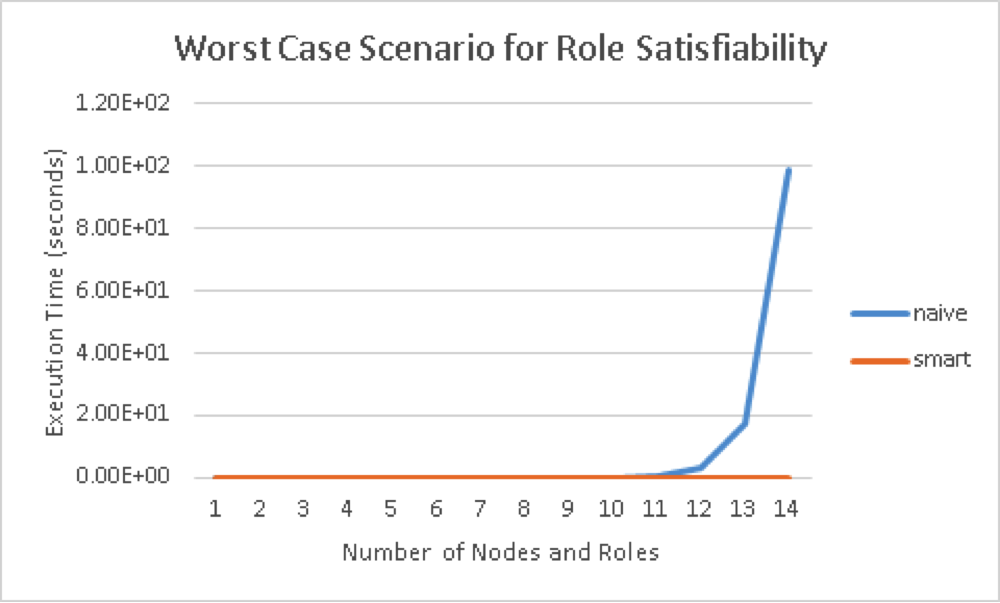
\includegraphics{fig1.png}}
\caption{Execution time for the worst-case scenario for role satisfiability; the smart algorithm outperforms the naive algorithm}
\end{figurehere}
\vspace{.1in}

\begin{figurehere}
\centering
\resizebox{\columnwidth}{!}{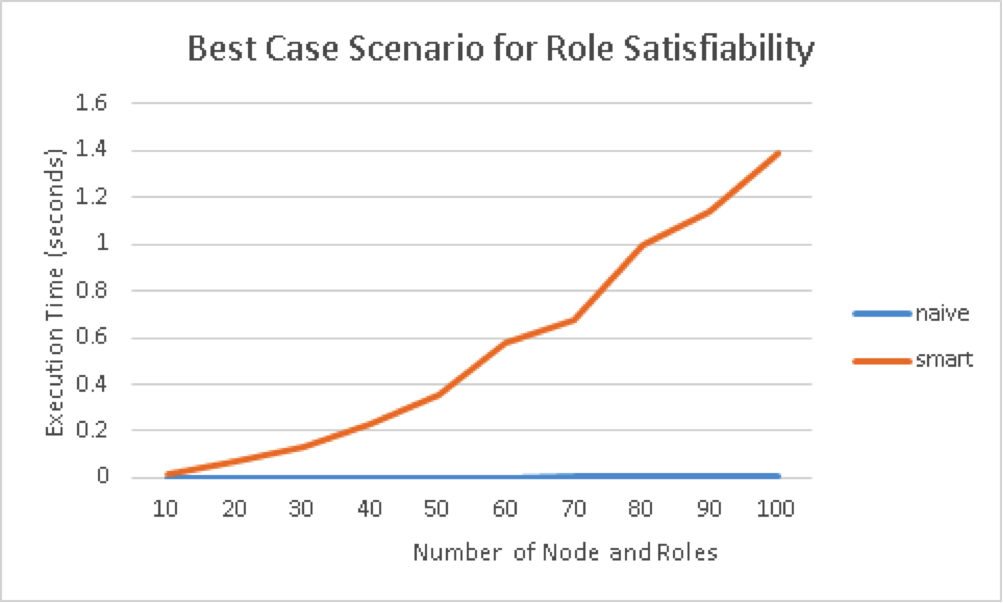
\includegraphics{fig2.png}}
\caption{Execution time for the best-case scenario for role satisfiability. The naive algorithm performs considerably better than the smart algorithm. However, the best-case scenario is rare -- these benefits are hard to come by in practice.}
\end{figurehere}
\vspace{.1in}

\begin{figurehere}
\centering
\resizebox{\columnwidth}{!}{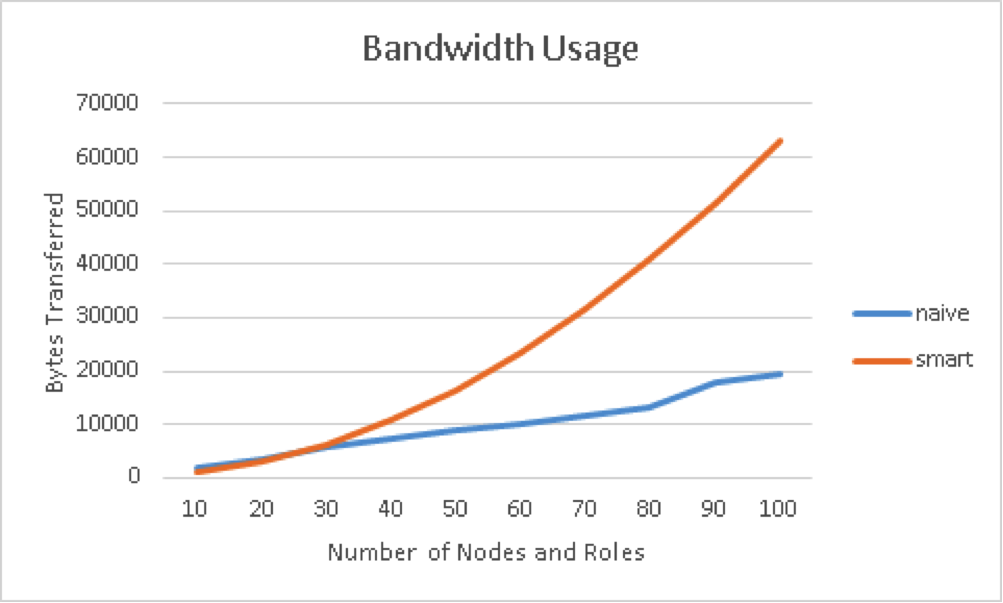
\includegraphics{fig3.png}}
\caption{The overall bandwidth usage across all nodes, including the server in the naive algorithm.}
\end{figurehere}
\vspace{.1in}

From \textit{Figure 1}, it is clear that the smart algorithm outperforms the naive algorithm. This is due to the exponential time complexity of the naive algorithm in the worst-case. The time that the smart algorithm spends in order to compute assignment flexibility allows it to overtake the naive algorithm for larger values of $|R|$. However, Figure 2 shows that the naive algorithm performs better than the smart algorithm in the best-case scenario. This is because the naive algorithm only has one role assignment to consider for every node and can assign those roles in linear manner. The smart algorithm, on the other hand, must notify every node in the assignment path each time a role is assigned. Since this happens for each node's role assignment, the smart algorithm's time complexity is quadratic in nature. Figure 3 also reflects the quadratic nature of the smart algorithm in terms of bandwidth usage: the token, which is linear in size, must be sent to each node for processing, and each newly chosen role must be broadcasted to every node in the assignment path. For the naive algorithm, the bandwidth usage is linear because each node must send its parameters to the server, and the server must send back a role assignment to each node.
\section{Algorithm Analysis}
The algorithm's message complexity is derived as follows: there are $|N| - 1$ messages for sending the token from node to node, and there are $|N|^2$  messages for creating and updating the token as roles are assigned to nodes. Because there can be more nodes than roles in the system, we must consider $|N|$ rather than $|R|$ in the worst-case. Thus, the algorithm produces $|N|^2 + |N| - 1$ messages.

The test results above suggest that algorithm's time complexity is quadratic in nature. However, this is somewhat misleading due to the fact that the results were obtained on a single machine using the SimulatedNetwork class. As a result, the benefits of parallelism are lost. Theoretically, the amount of work that each node must perform is $|R|$ for evaluating each role initially and $|R|$ for updating the assignment index for each role. Since $|N|$ work is required to transfer the token throughout the system and $|N|$, the overall work complexity is really $O(|R| + |N|)$.

The space complexity for each node is $O(|R|)$, because each node can satisfy at most $|R|$ roles. The space complexity for the token is $O(|N|)$, because the assignment path will initially contain all nodes in the system.

\section{Conclusion}
The naive centralized algorithm is grossly inefficient because it tries all possible role assignments in order to find one that works. Our algorithm uses the notions of flexibility and grading to efficiently assign roles to the best possible nodes while still avoiding open conflicts. Although the above test results indicate that the naive centralized algorithm performs better empirically in some metrics, the theoretical time complexity of our algorithm suggests that it is a better choice for large systems.

\section{Future Work}
One area of future work is improving the space efficiency of the token. Instead of storing the assignment path in the token, the assignment path can be computed on demand as each node receives the token. If a node computes an empty assignment path, the algorithm terminates.

Another area of future work is implementing a centralized version of our algorithm. Similar to the current version of the algorithm, each node would evaluate itself against $R$ in order to produce a set of tuples, each of which contains a satisfied role, flexibility, and grade. However, instead of computing an assignment index from that set and sending it to the root node, each node would send that set directly to a server node. The server node would be able to compute the assignment index for all nodes and make all role assignments in a centralized manner, without needing to send the ``Update Assignment Index'' messages to each node. The resulting algorithm may be more efficient than the current algorithm, although at the loss of decentralization.

Finally, our algorithm greedily chooses the best node at the time of each role assignment. An alternative version of the algorithm might choose the best possible assignment of all roles based on some cost function. However, such an algorithm would inherently need to be implemented using a branch and bound paradigm for efficiency.

\end{multicols}
\begin{thebibliography}{9}

\bibitem{aws}
  \emph{Amazon Elastic MapReduce}
  \url{http://s3.amazonaws.com/awsdocs/ElasticMapReduce/latest/emr-dg.pdf}

\bibitem{hadoop}
  J. Xie, S. Yin, Xi. Ruan, Z. Ding, Y. Tian, J. Majors, A. Manzanares, and X. Qin
  \emph{Improving MapReduce Performance through Data Placement in Heterogeneous Hadoop Clusters}
   Eng.auburn.ed. April 2010.
  \url{http://www.eng.auburn.edu/~xqin/pubs/hcw10.pdf}

\bibitem{iotivity}
  \emph{IoTivity}
  \url{https://www.iotivity.org}

\bibitem{azure}
  \emph{Azure IoT Suite}
  \url{https://www.microsoft.com/en-us/server-cloud/internet-of-things/azure-iot-suite.aspx}

\bibitem{loadb}
  S. Ludwig, A. Moallem
  \emph{Swarm Intelligence Approaches for Grid Load Balancing}
  J Grid Computing (2011)

\bibitem{mesh}
  Y. AMIR, C. DANILOV, R. MUSALOIU-ELEFTERI and N. RIVERA
  \emph{The SMesh Wireless Mesh Network}
  ACM Transactions on Computer Systems, Vol. 28, No. 3, Article 6, Publication date: September 2010.
  \url{http://www.cnds.jhu.edu/pub/papers/SMesh_ACM_TOCS_2010_09.pdf}

\bibitem{garg}
 V. Garg
 \emph{Concurrent and Distributed Systems in Java}
  A JOHN WILEY \& SONS, INC., PUBLICATION, 2004

\bibitem{MST}
  R. G. GALLAGER, P. A. HUMBLET, and P. M. SPIRA,
  \emph{A Distributed Algorithm for Minimum-Weight Spanning Trees},
  ACM Transactionson Programming Languages and Systems, Vol.5, No. 1, January 1983.
  \url{http://www.cs.tau.ac.il/~afek/p66-gallager.pdf}

\bibitem{rpyc}
  \emph{RPyC Unbounded Computing},
  \url{http://rpyc.readthedocs.org/en/latest/api/core_protocol.html}

\end{thebibliography}

\section{Appendix: Code Listings}
\appendix
\begin{center}
\textit{Full code listings and algorithm code in Python available at https://github.com/triskadecaepyon/DF\_RoleMatrix}\\
\vspace{3mm}
\large{\textbf{Listing A.1}}
\end{center}

\begin{algorithmic}
\State{node\_k::}
\State{$R:$ set of role criteria}
\State{$P:$ set of node parameters}
\State{$N:$ number of nodes}
\State{$S:$ set of satisfiable roles}
\State{grade: function that maps roles to grades}
\State{index: assignment index for the current node}
\end{algorithmic}

\begin{algorithmic}
\Function{BeginAssignment:}{}
   \State{token $:= CreateToken$()}
   \State{$ForwardToken$(token)}
\EndFunction
\end{algorithmic}

\begin{algorithmic}
\Function{CreateToken:}{}
   	\State{indices $:= \{\}$}
   	\For{dst $:= 1$ to $N$}
      		\State{$SendMessage$(dst, ``Compute Assignment Index'')}
      		\State{indices $:=$ indices $\cup$ $ReceiveMessage$(dst, ``Assignment Index Result'')}
   	\EndFor
	\State{path = $CreateAssignmentPath$(indices)}
   	\State{num\_roles\_to\_assign $:= |R|$}
   	\Return (path, num\_roles\_to\_assign)
\EndFunction
\end{algorithmic}

\begin{algorithmic}
\Function{CreateAssignmentPath:}{indices}
	\State{indices $:= sort\_ascending$(indices)}
   \State{indices $:= remove\_zero\_flexibility\_entries$(indices)}
	\Return{$map$(indices, $lambda$(index)(index.node\_id))}
\EndFunction
\end{algorithmic}

\begin{algorithmic}
\Function{UpdateToken:}{token, chosen\_role}
	\State $indices := \{\}$
	\For{dst $:= 1$ to $len$(token.path)}
		\State{$SendMessage$(dst, ``Update Assignment Index'', chosen\_role)}
		\State{indices $:=$ indices $\cup ReceiveMessage$(dst, ``Assignment Index Result'')}
	\EndFor
	\State{path $:= CreateAssignmentPath$(indices)}
	\Return{(path, token.num\_roles\_to\_assign $- 1$)}
\EndFunction
\end{algorithmic}

\begin{algorithmic}
\Function{ForwardToken:}{token}
	\State{next $:= pop\_first$(token.path)}
	\State{$SendMessage$(next, ``Token'', token)}
\EndFunction
\end{algorithmic}

\begin{algorithmic}
\Function{Upon receiving ``Token'' message:}{token}
	\If{$|S| > 0$}
		\State{chosen\_role $:= choose\_role$(S)}
		\State{$S := S -$ chosen\_role}
		\State{token $:= UpdateToken$(token, chosen\_role)}
	\Else
		\State{chosen\_role $:= NIL$}
	\EndIf
	\If{token.roles\_left $> 0$}
		\If{$len$(token.path) $> 0$}
			\State{$ForwardToken$(token)}
		\Else
         \State{$error$(``failed to assign all roles'')}
		\EndIf
	\Else
		\State{$success$(``all roles assigned'')}
	\EndIf
\EndFunction
\end{algorithmic}

\begin{algorithmic}
\Function{Upon receiving ``Compute Assignment Index'' message:}{src}
	\State{index $:= EvaluateRoles$()}
	\State{$SendMessage$(src, ``Assignment Index Result'', index)}
\EndFunction
\end{algorithmic}

\begin{algorithmic}
\Function{Upon receiving ``Update Assignment Index'' message:}{src, role}
	\If{role $\in S$}
		\State{$S := S -$ role}
		\State{index.flexibility $:=$ index.flexibility $- 1$}
		\If{index.flexibility $> 0$}
			\State{old\_grade $:= 1 / $ index.priority}
			\State{index.priority $:= 1 /$ (old\_grade $- grade$(role))}
		\Else
			\State{index.priority $:= \infty$}
		\EndIf
	\EndIf
	\State{$SendMessage$(src, ``Assignment Index Update'', index)}
\EndFunction
\end{algorithmic}

\begin{algorithmic}
\Function{EvaluateRoles:}{}
	\State{grade $:=  f: R \rightarrow \mathbb{R}$}
	\State{$S := \{r \in R :  grade (r) > 0\}$}
        \State{flexibility $:= |S|$}
        \If {flexibility $> 0$}
        		\State{priority $:= 1 / \sum_{r \in S }grade(r)$}
	\Else
		\State{priority $:= \infty$}
        \EndIf
        \State{node\_id $:= i$}

	\Return{(flexibility, priority, node\_id)}
\EndFunction
\end{algorithmic}

\begin{center}
\large{\textbf{Listing A.2}}
\end{center}

\lstset{frame=single, caption=Example Framework Listing in Python}
\begin{lstlisting}
import os, sys

lib_path = os.path.abspath(os.path.join('.', '..'))
sys.path.append(lib_path)

from logical_token import Token
from network import *
from logical_node import *
from role_criteria import *

class CompPowerRoleCriteria(RoleCriteria):

    # Note the global value must be more than 0 for the mul. masks to work
    __GLOBAL_ROLES_LIST__ = []
    __PROCESSING_POWER__ = 0
    __MEMORY_CAPABILITIES__ = 0
    __GPU_POWER__ = 0
    __NETWORK_SPEED__ = 0
    __STORAGE__CAP = 0
    __FLEX__ = 0
    __GRADE_VECTOR__ = []
    __ROLE__ = 0
    name = ""

    def __init__(self, grade_vector, name=""):
        #print('Created Container for Work unit')
        self.__GRADE_VECTOR__ = grade_vector
        self.__PROCESSING_POWER__ = self.__GRADE_VECTOR__[0]
        self.__MEMORY_CAPABILITIES__ = self.__GRADE_VECTOR__[1]
        self.__GPU_POWER__ = self.__GRADE_VECTOR__[2]
        self.__NETWORK_SPEED__ = self.__GRADE_VECTOR__[3]
        self.__STORAGE__CAP = self.__GRADE_VECTOR__[4]
        self.__generate_flexibility__()
        self.name = name

    def __generate_flexibility__(self):
        temp_grade = self.get_scalar_grade(self.__GRADE_VECTOR__)
        self.__FLEX__ = temp_grade

    def get_scalar_grade(self, role_grade_vector):
        """
        A very basic variant of flexibility grading (or the null method).
        Creates a grade on how flexible the system is to all types of task,
        such that priority is pivoted by flexibility ratings.
        """
        temp_grade = 0
        #print(self.__GRADE_VECTOR__[0])
        if role_grade_vector[0] > 0:
            temp_grade += role_grade_vector[0] * 3
        if role_grade_vector[1] > 1:
            temp_grade += role_grade_vector[1] * 2
        if role_grade_vector[2] > 1:
            temp_grade += role_grade_vector[2] * 2
        if role_grade_vector[3] > 1:
            temp_grade += role_grade_vector[3]
        if role_grade_vector[4] > 1:
            temp_grade += role_grade_vector[4]

        return temp_grade

    def get_my_grade(self):
        return self.__FLEX__

    def evaluate_against(self, node_parameters):
        """
        Used to compare roles from a 5 element list of values.
        Returns a binary list if the role is satisfied or not.
        """
        # Return a binary true if it can handle the role
        role_satisfy = [0, 0, 0, 0, 0]

        if self.__PROCESSING_POWER__ > node_parameters[0]:
            role_satisfy[0] = 1
        if self.__MEMORY_CAPABILITIES__ > node_parameters[1]:
            role_satisfy[1] = 1
        if self.__GPU_POWER__ > node_parameters[2]:
            role_satisfy[2] = 1
        if self.__NETWORK_SPEED__ > node_parameters[3]:
            role_satisfy[3] = 1
        if self.__STORAGE__CAP > node_parameters[4]:
            role_satisfy[4] = 1

        # return role_satisfy

        # At least 3 of the functionality thresholds are met
        if role_satisfy.count(1) >= 3:
            return 1
        else:
            # Even if 3 aren't met, I have enough capabilities
            # to get something done
            if self.get_scalar_grade(self.__GRADE_VECTOR__)
            	>= self.get_scalar_grade(node_parameters):
                return 1
            else:
                return 0

# Clients will define their own RoleCriteria, which will expect
# a certain set of parameters to evaluate on
role_criterias = [
    CompPowerRoleCriteria([1, 1, 5, 2, 5], "Mobile"),
    CompPowerRoleCriteria([2, 3, 1, 2, 5], "Desktop"),
    CompPowerRoleCriteria([5, 5, 5, 5, 5], "Server")
]

nodes = [
    LogicalNode(0, [1, 1, 1, 1, 1], role_criterias),
    LogicalNode(1, [2, 2, 2, 2, 2], role_criterias),
    LogicalNode(2, [3, 3, 3, 3, 3], role_criterias),
    LogicalNode(3, [4, 4, 4, 4, 4], role_criterias)
]

network = SimulatedNetwork(nodes)

token = nodes[0].begin_logical_assignment()

if token:
    print "Error! Some roles couldn't be satisfied"
    for role_id in token.unassigned_roles:
        print "Role %d: %s" % (role_id, role_criterias[role_id].name)
else:
    print "Success! All roles assigned!"
    for node in nodes:
        if node.assigned_role is not None:
            print "Node %d's role: %s" % (node.node_id,
            	role_criterias[node.assigned_role].name)

\end{lstlisting}


\end{document}